\RequirePackage{fixltx2e} %This package in CTeX is not compatible with revtex4-1
\documentclass[aps,pre,12pt,preprint,onecolumn,showpacs,showkeys]{revtex4-1}
\usepackage{ctex}
\usepackage{mathtools,mathrsfs}
\usepackage{multirow}
\usepackage{setspace,dcolumn}
\usepackage{hyperref}
\usepackage{graphicx,psfrag,epsfig}
\usepackage[font=small,format=plain,labelfont=bf,textfont=it,justification=centering,singlelinecheck=false]{caption}
\usepackage{amsmath,amsfonts,amssymb,amsthm,bm,upgreek}
\usepackage{geometry}
\usepackage[mathscr]{eucal}
\usepackage{caption}
\usepackage{subcaption}
\hypersetup{colorlinks=true}
\geometry{top=2.54cm,bottom=2.54cm,left=3cm,right=3cm}
\renewcommand\appendixname{附录}
\renewcommand\abstractname{}%摘要
\renewcommand\tablename{表}
\renewcommand\figurename{图}
\makeatletter
\def\@pacs@name{\songti\zihao{-4}{\bf PACS码:}}
\def\@keys@name{\songti\zihao{-4}{\bf 关键词:}}
\def\Dated@name{日期:}
\def\Received@name{\zihao{-5}{接收} }
\def\Revised@name{\zihao{-5}{修订} }
\def\Accepted@name{\zihao{-5}{采纳} }
\def\Published@name{\zihao{-5}{发表} }
\makeatother
\linespread{1.3}
\renewcommand{\labelenumi}{\alph{enumi}.}
\leftmargini=20mm
\def \d {\mathrm d}
\def \degree {^\circ}
\def \V {\bm{V}}
\def \degC {^\circ \mathrm{C}}

\begin{document}
\title{\bf\heiti\zihao{3}电子衍射\vspace{15mm}}
\author{\fangsong\zihao{4}邵智轩\vspace{2mm}}
\affiliation{\songti\zihao{-4}学号:1400012141\vspace{2mm}}
\date{\today}
%\pacs{02.10.Yn, 33.15.Vb, 98.52.Cf, 78.47.dc}
\keywords{电子衍射,反射球,单晶,多晶,倒格矢,晶格常量}
\email{shaozhixuansh@pku.edu.cn; (86)13381350619}

\begin{abstract}
\vspace{10mm}
\begin{spacing}{1.5}
\songti\zihao{-4}
    本实验学习使用透射电子显微镜(TEM),观察了单晶和多晶的衍射图样,以及样品的微观形貌。在定量方面,通过已知晶格常量的Au多晶样品标定了$\sin \theta - D$曲线,进而测量了Ag 和 Cu 多晶样品和Si单晶样品的晶格常数。

\end{spacing}
\end{abstract}
\maketitle
\songti\zihao{-4}

\section{引言}
    德布罗意在1924年提出微观粒子具有波粒二象性,并提出了著名的德布罗意关系:
    \begin{eqnarray}
        E=h\nu\\
        p=\frac{h}{\lambda}\bm{n}=h\bm{k}
    \end{eqnarray}
    由此可求得电子的德布罗意波长$\lambda$(单位:0.1 nm)和加速电压$V$(单位:V)之间的关系:
    \begin{equation}\label{eq:debr}
        \lambda=\frac{h}{p}=\frac{h}{\sqrt{2 m E}}=\frac{h}{\sqrt{2 m e V}}=\sqrt{\frac{150}{V}}
    \end{equation}
    1927 年戴维孙和革末把电子注射到镍单晶上,所得到的结果与X射线的衍射现象完全相同。由衍射图形求得的入射电子波长与式(\ref{eq:debr})符合得很好,就从实验上证实了德布罗意的假设。

    由于电子在物质中的穿透深度很小,它更适合用来研究微晶、表面和薄膜的晶体结构。对于加速电压几十到几百伏的低能电子,它对样品的穿透能力较弱,只有表面几层的原子对衍射图像有贡献,因此低能电子衍射已成为表面结构分析的有力手段。

    本实验的目的式掌握电子衍射的运动学理论,用它来研究单晶与多晶的衍射现象。

\section{原理}
    \subsection{原子对电子的弹性散射}
        量子力学中,原子对电子的散射可用薛定谔方程描述:
        \begin{equation}\label{eq:Schr}
            \nabla ^2 \psi (\bm r) + \frac{2 m}{h^2}[E-e \phi _a (\bm r)]\psi (\bm r)=0
        \end{equation}
        当电子在原子势场中的能量 $ e \phi _a(\bm r)$比入射电子能量小得多时,我们可以把势能$ e \phi _a(\bm r)$ 看作微扰。这时式(\ref{eq:Schr})的一般解为:
        \begin{equation}\label{eq:gen_sol}
            \psi(\bm r)=\psi _0 (\bm r)+f _e (\bm s)\cdot \frac{\exp(i 2 \pi \bm{k}_0 \cdot \bm r)}{r}
        \end{equation}
        其中$\bm s = \bm k - \bm k_0$。式(\ref{eq:gen_sol})等号右边第一项为入射平面波,第二项表示由原子散射所引起的向各个方向传播的散射波,它可以看成是以原子为中心向不同方向散射的,波矢大小仍为$k_0$的球面波(只讨论弹性散射)。$f_e(\bm s)$决定了向不同方向散射的球面波振幅之间相互关系,称为原子散射因子。根据波恩一级近似有:
        \begin{equation}\label{eq:scatter}
            f_e(\bm s)=\frac{2 \pi m e}{h^2}\int \phi _a (\bm r)\exp[i 2 \pi \bm{s}\cdot \bm {r}]=\frac{2 \pi m e }{h^2}\mathcal{F}\{\phi _a (\bm r)\}
        \end{equation}
        即$f_e(\bm s)$正比于原子势场的傅里叶变换。而电子在各个方向上散射的强度正比于$|f_e(\bm s)|^2$。
    \subsection{晶胞对电子的散射}
        晶胞势场$\phi_0(\bm r)$,它等于晶胞中各原子的势场之和:
        \begin{equation}\label{eq:periodic_potential}
            \phi _0 (\bm r)=\sum_j \phi _j (\bm{r}-\bm{r}_j)
        \end{equation}
        将式(\ref{eq:periodic_potential})带入式(\ref{eq:scatter}),即得晶胞对电子的散射:
        \begin{eqnarray}\label{eq:cell_factor}
            F(\bm s)&=& \frac{2 \pi m e }{h^2}\int\left[\sum _j \phi _j (\bm r- \bm r _j)\right]\cdot \exp[i 2 \pi (\bm k - \bm k_0)\cdot \bm r]\d \bm r \nonumber \\
            &=&\sum_j f_0^j (\bm s) \cdot \exp[i 2\pi \bm s \cdot \bm r _j]
        \end{eqnarray}
        式中$f_0^j$为晶胞中第$j$个原子的散射原子,指数中的因子$2\pi (\bm k -\bm k_0)\cdot \bm r_j$ 反映位矢为$\bm r_j$的原子与原点处原子的散射波的相位差。式(\ref{eq:cell_factor})表示晶胞对电子的散射等于晶胞中所有原子对入射电子散射的相干叠加,$F$称为晶胞的结构振幅,$|F|^2$则给出了不同方向上晶胞对电子散射的强度。
    \subsection{单晶对电子的衍射}
        对于晶体来说,某一方向的衍射束是处于不同位置的晶胞对于入射电子散射的相干叠加,其结果使得在一定的方向才存在衍射束(衍射加强),而在其他方向上则不存在衍射(衍射相消)。晶体衍射加强的条件,由劳厄方程给出:
        \begin{equation}
            \bm s=\bm k - \bm k_0= h \bm{a}^*+k \bm{b}^*+l \bm{c}^*
        \end{equation}
        即只有当波矢差等于某个倒格矢的时候,才出现相干相长。
    \subsection{反射球与指标化方法}\label{sec:indices}
        \begin{figure}[ht]
        \centering
        \includegraphics[width=75mm]{fansheqiu}
        \caption{\label{fig:fansheqiu}%
        由衍射斑求对应的晶面族的面间距$d_{hkl}$}
        \end{figure}
        在倒空间中可以引入反射球,即在倒空间的原点O 沿入射波矢方向做一矢量使其由L点指向O点,长度为$\frac{1}{\lambda}$,再以L为球心,$\frac{1}{\lambda}$为半径作一球,则落在球面上的倒格点与球心$L$连线的方向满足衍射加强的条件。由于电子波长$\lambda$很短(0.04$\sim$0.06 \AA),$\frac{1}{\lambda}$比倒格矢基矢大得多,二者相差几十倍。如果我们在垂直入射电子方向放一底片,该底片与上述反射球平行,这时入射束和衍射束与底片的交点正好与反射球面上倒格点的位置相对应,因此我们所得到的电子衍射图形与在O点所作的与入射束方向垂直的二维截面上的倒格点的图形相似。如图(\ref{fig:fansheqiu})所示,有几何关系:
        \begin{equation}
            \frac{1}{\lambda}:L_0=g_h:\overline{O'G'}
        \end{equation}
        对于电子衍射,由于波长很短,衍射角也很小,一般小于$3\degree$,上式中的$\overline{O'G'}$可以用底片上$O'$与$G''$之间的距离$R_c$代替,从而有
        \begin{equation}
            L_0 \lambda \approx R_c \cdot d_{hkl} 
        \end{equation}
        根据图(\ref{fig:fansheqiu}),进而有
        \begin{eqnarray}
            \sin \theta &=&\frac{\lambda}{2 d_{hkl}}\\
            &=&\frac{\lambda \sqrt{h^2+k^2+l^2}}{2 a_0}\label{eq:bragg}\\
            &\approx& \frac{R_c}{2 L_0}
        \end{eqnarray}
        其中$a_0$ 为所测量晶体的晶格常数。

        在使用相同能量(固定电压)的电子束时,$\lambda$ 为确定常数。在本实验的实验装置中,样品与底片之间存在着中间镜,各衍射斑对应的衍射角不能直接通过$R_c$和$L_0$得出,可用已知结构和晶格常量的定标样品,通过做定标曲线得到$R_c$与$\sin \theta$的关系。定标后,可测量实验中待测样品的衍射环直径$D=2R_c$,从$\sin \theta - D$曲线上得到所对应的$\sin \theta $值,进而可求得晶面间距$d_{hkl}$。再通过指标化方法(教材195页)同时确定晶面指数$(h,k,l)$和晶格常量$a_0$。
    \subsection{多晶的衍射图样}
        在多晶中,晶胞的取向在各个方向的概率完全相同,故衍射图样是许多同心的圆环,称为德拜环,同样可以用\ref{sec:indices}中提到的指标化的方法来进行分析。
\section{实验装置}
    \begin{figure}[ht]
	\centering
	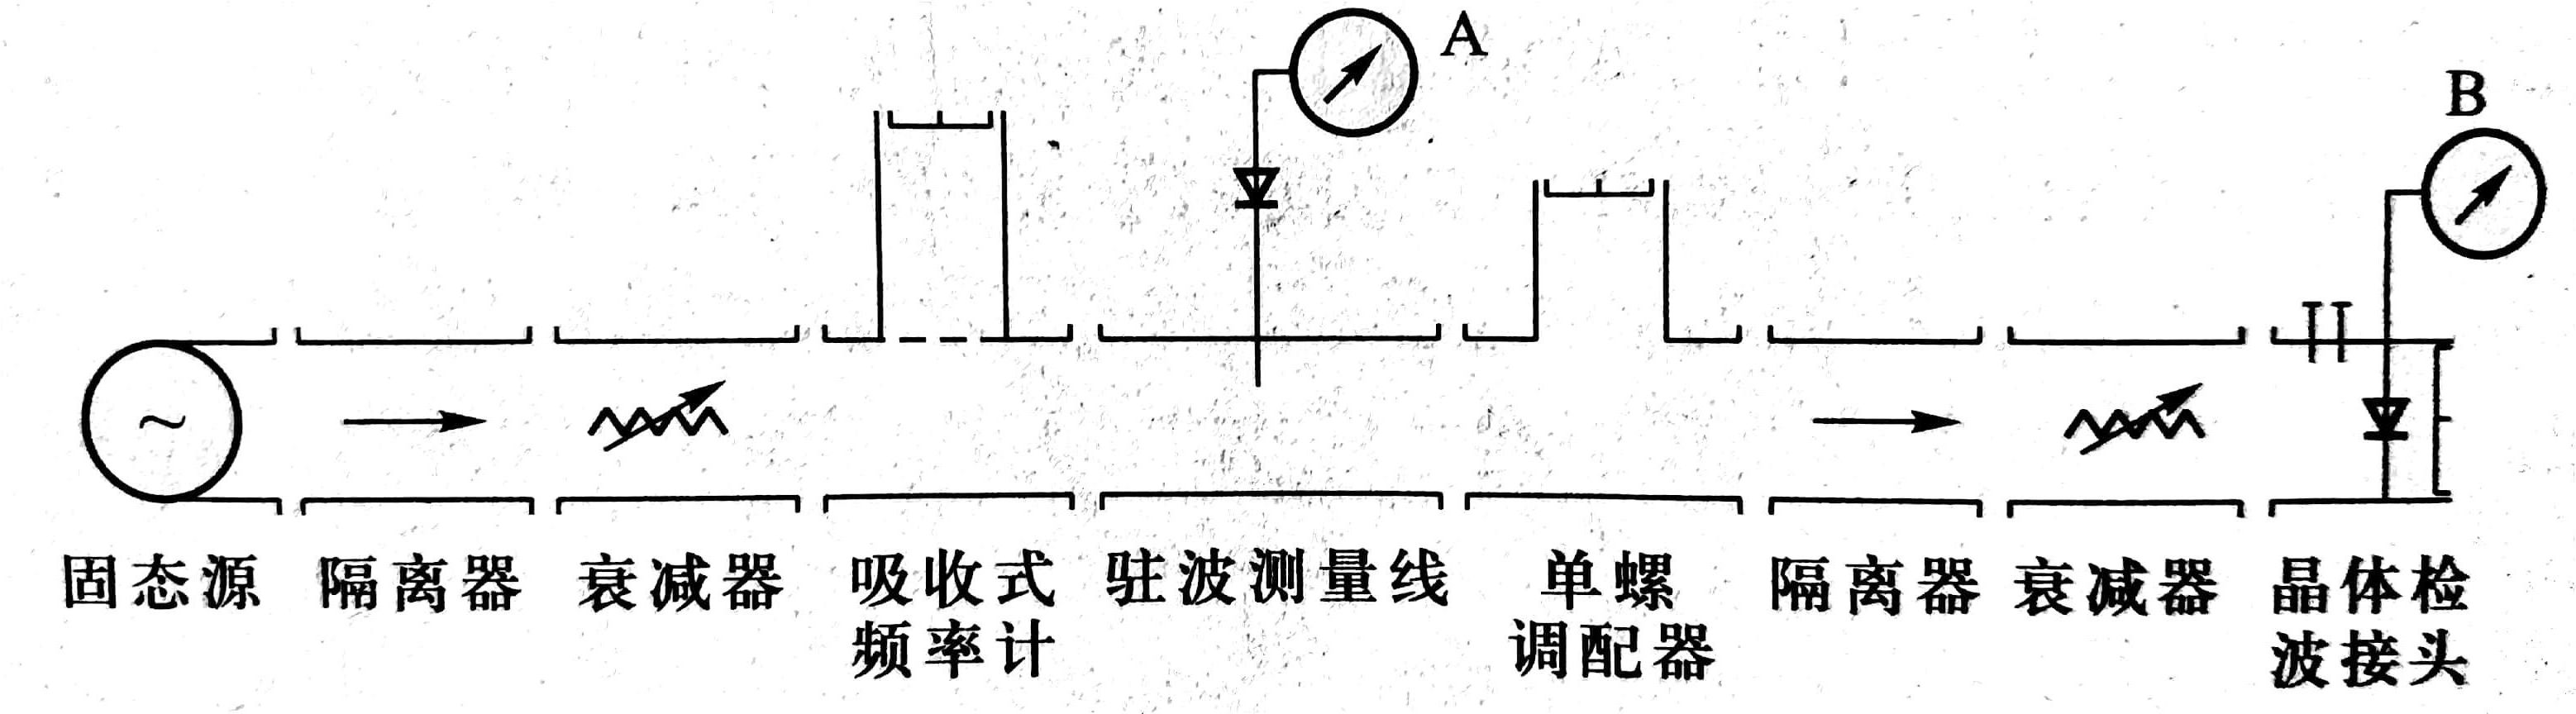
\includegraphics[width=75mm]{equip}
	\caption{\label{fig:equip}%
	透射电镜内部结构示意图}
	\end{figure}
    本实验中所用的电子衍射装置为透射电子显微镜,图(\ref{fig:equip})为其结构示意图。阴极发射热电子,经加速电压加速后进过一系列电磁透镜及光阑汇聚到所选择的样品区域上,透过样品时发生衍射,之后再用电磁透镜进行焦面接收并放大成像至荧光屏上,屏下可填装胶片进行拍摄。整个系统需工作在$10^{−3}\,\mathrm{Pa}$ 以下的真空下,故使用机械泵和扩散泵的二级真空系统。

    实验中所采用的样品采用沉积法制备,即将材料在真空中加热,使其蒸气沉积在NaCl 晶体衬底上形成薄膜,喷镀后溶于水就可以脱落形成薄膜,再将其置于铜网上,干燥后即可观察。

\section{实验内容}
    实验中所采用的定标样品为 Au 的多晶样品,待测样品为Ag、Cu 的多晶样品以及Si的单晶样品。
    \begin{enumerate}
        \item 拍摄Au 多晶样品的德拜相及形貌像,测量衍射环的直径作为定标样品。
        \item 拍摄其余三样品的衍射图样及其中两多晶样品个的形貌图样,利用指标化的方法进行处理,得到其结构以及晶格常数。
    \end{enumerate}

\section{实验结果}
    本实验中电子加速电压均为$160\,\mathrm{kV}$,利用式(\ref{eq:debr}),$\lambda=0.030619\,\text{\AA}$。
    \begin{figure}[ht]
	\centering
		\begin{subfigure}[t]{75mm}
			\centering
			\includegraphics[width=75mm]{19_cropped}
			\caption{Ag多晶}\label{fig:19}
		\end{subfigure}
		\begin{subfigure}[t]{75mm}
			\centering
			\includegraphics[width=75mm]{22_cropped}
			\caption{Cu多晶}\label{fig:22}
		\end{subfigure}
		\begin{subfigure}[t]{75mm}
			\centering
			\includegraphics[width=75mm]{29_cropped}
			\caption{Au多晶}\label{fig:29}
		\end{subfigure}
		\begin{subfigure}[t]{75mm}
			\centering
			\includegraphics[width=75mm]{32_cropped.jpg}
			\caption{Si单晶}\label{fig:32}
		\end{subfigure}
		\caption{各样品的衍射图样}\label{fig:yanshe}
    \end{figure}
    实验所摄的衍射图样如图(\ref{fig:yanshe})所示。

    首先利用Au多晶(面心立方)样品进行定标,作校准曲线。Au的晶格常量$a_0=4.0786\text{\AA}$,各衍射环对应的晶面指数$(h,k,l)$,相应的$h^2 +k^2+ l^2$、$\sin \theta$,以及实际用尺子测量的各衍射环的直径$D$如表\ref{tab:Au}所示。

    \begin{table}[h]
		\caption{\label{tab:Au}%
		Au 薄膜样品各衍射环的$\sin \theta - D$ 关系}
		\begin{tabular}{|c|c|c|c|c|}
			\hline
			环序&$hkl$&$h^2+k^2+l^2$&衍射环直径$D$(mm)&$\sin \theta$\footnote{由式(\ref{eq:bragg}),$\sin \theta=\sqrt{h^2+k^2+l^2}\frac{\lambda}{2 a_0}=\sqrt{h^2+k^2+l^2}\times 3.75357\times 10^{-3}$}\\\hline
            1 & 111&  3 &  20.0 &  0.006501 \\\hline 
            2 & 200&  4 &  23.6 &  0.007507 \\\hline
            3 & 220&  8 &  33.0 &  0.010617 \\\hline
            4 & 311& 11 &  38.5 &  0.012449 \\\hline
            5 & 222& 12 &  40.0 &  0.013003 \\\hline
            6 & 400& 16 &  51.6 &  0.015014 \\\hline
            7 & 331& 19 &  57.5 &  0.016361 \\\hline
            8 & 420& 20 &  61.0 &  0.016786 \\\hline
            9 & 422& 24 &  69.8 &  0.018389 \\\hline
        \end{tabular}
	\end{table}
    \begin{figure}[ht]
        \centering
        \includegraphics[width=100mm]{dingbiao}
        \caption{\label{fig:dingbiao}%
        利用已知的Au晶格常数作$\sin \theta -D$校准曲线,图中点的数据来源于表\ref{tab:Au}}
    \end{figure}
    在图(\ref{fig:dingbiao})中我们看到,线性关系似乎并不是那么好,所以在后续数据处理中,用分段线性插值的方法来确定于$D$相应的$\sin\theta$。

    \begin{table}[h]
		\caption{\label{tab:Ag}%
		Ag 薄膜样品各衍射环的直径$D$,相应的$\sin \theta$,以及计算得到的$a_0$}
		\begin{tabular}{|c|c|c|c|c|c|}
			\hline
			环序&$hkl$&$h^2+k^2+l^2$&$D$(mm)&$\sin \theta$&$a_0$(\AA)\footnote{由式(\ref{eq:bragg}),$a_0/\lambda=\frac{\sqrt{h^2+k^2+l^2}}{2 \sin \theta}$}\\\hline
            1 & 111&  3 &  20.5 &  0.006641 &3.9928\\\hline 
            2 & 200&  4 &  23.6 &  0.007507 &4.0786\\\hline
            3 & 220&  8 &  33.6 &  0.010817 &4.0032\\\hline
            4 & 311& 11 &  39.0 &  0.012634 &4.0190\\\hline
            5 & 222& 12 &  40.8 &  0.013089 &4.0510\\\hline
            6 & 400& 16 &  52.5 &  0.015220 &4.0235\\\hline
            7 & 331& 19 &  58.2 &  0.016446 &4.0575\\\hline
            8 & 420& 20 &  61.5 &  0.016878 &4.0566\\\hline
            9 & 422& 24 &  70.5 &  0.018516 &4.0503\\\hline
            &&&&&4.0370\\\hline
        \end{tabular}
    \end{table}

    \begin{table}[h]
		\caption{\label{tab:Cu}%
		Cu 薄膜样品各衍射环的直径$D$,相应的$\sin \theta$,以及计算得到的$a_0$}
		\begin{tabular}{|c|c|c|c|c|c|}
			\hline
			环序&$hkl$&$h^2+k^2+l^2$&$D$(mm)&$\sin \theta$&$a_0$(\AA)\footnote{由式(\ref{eq:bragg}),$a_0/\lambda=\frac{\sqrt{h^2+k^2+l^2}}{2 \sin \theta}$}\\\hline
            1 & 111&  3 &  19.2 &  0.006278 &4.2238\\\hline 
            2 & 200&  4 &  22.5 &  0.007200 &4.2527\\\hline
            3 & 220&  8 &  31.7 &  0.010817 &4.2507\\\hline
            4 & 311& 11 &  37.1 &  0.011983 &4.2374\\\hline
            5\footnote{这个环太模糊} & 222&12  &   &   &\\\hline
            6 & 400& 16 &  48.5 &  0.014477 &4.2301\\\hline
            &&&&&4.2389\\\hline
        \end{tabular}
    \end{table}
    
    通过指标化方法,得到Ag 和 Cu 都是面心立方结构;计算得Ag的晶格常数 4.0370\AA (实际值4.086 \AA),Cu的晶格常数 4.2389 \AA (实际值3.615 \AA)。其中Cu的晶格常数与实际值相差很远,这令我非常不解。原因可能有:
    \begin{enumerate}
        \item 标错了胶片序号,即我拿到的并不是Cu样品,仍是Ag 样品。
        \item 样品拍摄条件不够好、冲洗的时候操作不当,导致我这张照片的清晰度较低,有些环没有辨识出来。
        \item Cu相比Ag 和 Au,化学性质更活泼,长期暴露在空气中可能被氧化形成 CuO,使得晶格结构改变。形成了这样具有接近于简单立方格子嵌套结构的CuO 晶体,一方面每个原子的散射振幅相干形成了接近于体心立方格子的衍射图样,另一方面由于O 原子和Cu 原子的散射能力不同,在(111) 及(311) 晶面上同样形成了强度可分辨的散射束。最终测得的结果为CuO的三个晶格常数的平均。
    \end{enumerate}

    单晶Si的衍射图样如图(\ref{fig:32}),是六边形点阵,数据如表\ref{tab:Si},测得单晶Si的晶格常数5.6562 \AA ,与理论值 5.6575 \AA 相符合。
    
    \begin{table}[h]
		\caption{\label{tab:Si}%
		Si 单晶样品各衍射环的直径$D$,相应的$\sin \theta$,以及计算得到的$a_0$}
		\begin{tabular}{|c|c|c|c|c|c|}
			\hline
			环序&$hkl$&$h^2+k^2+l^2$&$D$(mm)&$\sin \theta$&$a_0$(\AA)\\\hline
            1 & 220&  8 &  24.6 &  0.007838 &5.5245\\\hline 
            2 & 422& 24 &  42.7 &  0.013471 &5.5675\\\hline
            3 & 440& 32 &  50.0 &  0.014737 &5.8765\\\hline
            &&&&&5.6562\\\hline
        \end{tabular}
    \end{table}


    \begin{figure}[ht]
        \centering
        \includegraphics[width=100mm]{27_cropped}
        \caption{\label{fig:27}%
        Au多晶薄膜的微观形貌像}
    \end{figure}

    此外还观察了以上各个样品的微观形貌。我拿回来的是Au形貌照片,如图(\ref{fig:27})所示。从图上可以清晰地看到Au多晶薄膜上的微观形貌。

\section{总结}
    本实验学习了电子衍射所涉及的动力学和固体物理学原理,并学习了透射电子显微镜(TEM)的使用方法。观察了单晶和多晶的衍射图样,以及样品的微观形貌。在定量方面通过已知晶格常量的Au多晶样品标定了$\sin \theta - D$曲线,通过指标化方法确定了Ag和Cu样品都是面心立方结构;Ag 的晶格常数为 4.0370 \AA,Cu 的晶格常数为4.2389 \AA,Cu的晶格常数明显违背于理论值,在文中给出了可能的原因。还测量了单晶Si的晶格常数:5.6562 \AA。

\section{致谢}
    感谢贾春燕老师对实验的悉心指导,对操作步骤的耐心讲解。
	
\begin{thebibliography}{}
\bibitem{Book} 吴思诚, 荀坤. 近代物理实验(第四版). 北京:高等教育出版社, 2015
\end{thebibliography}
\clearpage
\appendix
\section{实验报告思考题}
	\subsection{电子衍射和X射线衍射有何异同?}
        同:
        \begin{enumerate}
            \item 电子衍射的几何学与X 射线衍射完全一样,都遵循劳厄方程和布拉格方程所规定的衍射调教和几何关系。
            \item 电子衍射与X 射线衍射都是表征晶体结构的重要手段。
        \end{enumerate}

        异:
        \begin{enumerate}
            \item X 射线衍射中,轻原子对其的散射与重原子相比可以忽略,而在电子衍射中,轻原子对电子的散射和重原子相比有可比你的散射强度,使得电子衍射更有利于研究轻原子的分布。
            \item 由于电子的波长相对于X 射线较短,根据布拉格方程其衍射角也很小,使得单晶的电子衍射图样和其倒格子的一个二维截面分布相似,更加直观方便。
            \item 物质对电子的散射相对X 射线散射要强104 量级,使得衍射电子束的强度很高,忽略两次以上散射的运动学理论在许多情况下不再适用。
            \item 电子在物质中的穿透深度很小,因此更适合用于对微晶、薄膜以及晶体表面进行结构表征。
        \end{enumerate}

        
	
    \subsection{电子衍射实验中,为何要用指标化方法来处理实验数据?是否可以用其他方法来获得晶格类型和晶格常量?}
        对于一个未知的样品,利用指标化的方法能够较为方便,快速地分析出晶体的晶格类型,从而进一步确定晶体的晶格常量等信息。指标化方法一次就能判断晶格类型而不需要做对类型的假设 并计算验证 。
		
	

\end{document}